\documentclass[11pt,final,5p,times,twocolumn,authoryear]{elsarticle}
\usepackage[utf8]{inputenc}
\usepackage[T1]{fontenc}
\usepackage[spanish]{babel}
\usepackage{amsmath,amssymb,booktabs,graphicx,url,microtype}
\usepackage[hidelinks]{hyperref}
\addto\captionsspanish{\renewcommand{\tablename}{Tabla}}
\Urlmuskip=0mu plus 1mu
\begin{document}
\begin{titlepage}
    \centering
    {\Huge \bfseries Comparación de esquemas numéricos para un modelo farmacocinético no lineal de un compartimento\par}
    \vspace{0.5cm}
    
\includegraphics[width=0.45\textwidth]{UTEC-Logo.jpg}
    \par
    \vspace{0.5cm}
    {\Large \bfseries Integrantes:\par}
    \vspace{0.5cm}
    {\large Dávila Segovia, Giancarlo (202510521) \par}
    {\large Espinoza Torres, Hector Miguel (202410205) \par}
    {\large De la Cuba Palacios, Fabrizzio Alexander (202510737) \par}
    {\large Torres Caceres, Samantha Kristhin (202510712) \par}
    {\large Auqui Perez, Adrian Antonio (202120101) \par}
    \vspace{1cm}
    {\Large \bfseries Curso:\par}
    \vspace{0.5cm}
    {\large CC2104 Métodos Numéricos \par}
    \vspace{1cm}
    {\Large \bfseries Docente:\par}
    \vspace{0.5cm}
    {\large Patricia Reynoso Quispe \par}
    \vfill
    {\large \textbf{Barranco, 18 de octubre de 2026} \par}
\end{titlepage}

\begin{frontmatter}


\title{Comparación de esquemas numéricos para un modelo farmacocinético no lineal de un compartimento}


\author[utec]{G. Dávila}
\author[utec]{H. M. Espinoza}
\author[utec]{F. A. De la Cuba}
\author[utec]{S. K. Torres}
\author[utec]{A. A. Auqui}

\affiliation[utec]{organization={Universidad de Ingeniería y Tecnología (UTEC), Dirección de Ciencias},
            city={Lima},
            country={Perú}}

\begin{abstract}
Se comparan los métodos de Euler explícito, Euler implícito, Runge--Kutta de cuarto orden (RK4) y diferencias finitas no estándar (NSFD) en un modelo farmacocinético monocompartimental con eliminación de Michaelis--Menten. Se consideran condiciones iniciales y parámetros normalizados, cinco tamaños de paso y una referencia analítica basada en la función $W$ de Lambert. RK4 presenta el menor error máximo al refinar la malla, mientras que Euler explícito produce valores negativos con pasos gruesos. Una variación unifactorial de $C_0$, $V_{max}$ y $K_m$ permite comparar la respuesta de los cuatro esquemas y evidencia que la preservación de la positividad depende tanto del método como de los parámetros. Los indicadores de concentración y exposición se analizan junto con el costo de cálculo, estimado mediante 300 repeticiones de cada simulación, distinguiendo precisión cuantitativa y admisibilidad física.
\end{abstract}


\begin{keyword}
farmacocinética \sep Michaelis--Menten \sep Euler implícito \sep Runge--Kutta \sep diferencias finitas no estándar
\end{keyword}


\end{frontmatter}
\fontsize{11}{13.2}\selectfont


\section{Introducción}
\label{introduction}

La farmacocinética constituye una herramienta fundamental para comprender cómo cambia la concentración de un fármaco en el organismo a lo largo del tiempo y, por ello, permite relacionar una dosis administrada con procesos como la distribución y la eliminación. Dentro de este campo, los modelos farmacocinéticos monocompartimentales representan una aproximación matemática sencilla y útil, ya que consideran al organismo como un único compartimento en el que el medicamento se distribuye de manera homogénea. Aunque esta simplificación facilita el análisis, el comportamiento del sistema puede volverse considerablemente más complejo cuando la eliminación del fármaco deja de ser lineal y depende de la propia concentración, como ocurre en modelos basados en la cinética de Michaelis-Menten \citep{tang2007}. La solución puede obtenerse a partir de una relación implícita y expresarse mediante la función $W$ de Lambert \citep{wagner1973}. Aun así, los métodos numéricos permiten calcular la concentración paso a paso y estudiar las diferencias que aparecen al variar el tamaño de paso. Por lo tanto, el uso de métodos numéricos adquiere especial importancia. Sin embargo, no todos los métodos ofrecen el mismo desempeño: dependiendo del tamaño de paso y de las características del problema, algunos esquemas tradicionales pueden generar oscilaciones, pérdida de estabilidad o incluso valores negativos de concentración, los cuales carecen de sentido físico dentro de un modelo farmacocinético \citep{egbelowo2018}. Esta dificultad vuelve relevante el estudio de alternativas como los esquemas de diferencias finitas no estándar (NSFD), desarrollados para reproducir de manera más fiel ciertas propiedades cualitativas del modelo continuo, entre ellas la positividad y la estabilidad de las soluciones \citep{mickens2002}. Por esta razón, comparar distintos esquemas numéricos en un modelo monocompartimental con eliminación no lineal no constituye únicamente un ejercicio matemático, sino un problema con interés aplicado: una aproximación numérica poco adecuada puede distorsionar la interpretación de la evolución temporal de un medicamento y afectar parámetros que dependen directamente de la curva concentración-tiempo. Además, la literatura ha mostrado que estos modelos pueden estudiarse bajo distintas vías de administración y que su comportamiento numérico cambia según los parámetros y condiciones empleadas \citep{egbelowo2017, egbelowo2018}. En consecuencia, analizar la estabilidad y el comportamiento de diferentes métodos resulta relevante para identificar qué esquemas permiten obtener aproximaciones consistentes, físicamente razonables y suficientemente robustas para representar sistemas farmacocinéticos no lineales.

Diversos estudios han abordado la modelación farmacocinética y el desarrollo de métodos numéricos capaces de preservar las propiedades del sistema continuo. \citet{tang2007} analizaron un modelo farmacocinético monocompartimental con eliminación no lineal de tipo Michaelis–Menten, proporcionando una base matemática para describir la evolución de la concentración del fármaco. Posteriormente, \citet{egbelowo2017} aplicaron esquemas de diferencias finitas no estándar a un modelo farmacocinético lineal, mostrando su utilidad para mantener propiedades cualitativas de la solución. \citet{egbelowo2018} extendió este enfoque a modelos monocompartimentales con eliminación no lineal y distintas vías de administración, destacando que algunos métodos convencionales pueden presentar oscilaciones o valores físicamente inconsistentes cuando se emplean tamaños de paso inadecuados. Estos trabajos se apoyan en los principios desarrollados por \citet{mickens2002}, quien propuso los esquemas de diferencias finitas no estándar como una alternativa para preservar propiedades como la positividad y la estabilidad de las soluciones numéricas.

Estos antecedentes muestran que la representación numérica de modelos farmacocinéticos no lineales no depende únicamente de obtener una aproximación de la solución, sino también de conservar propiedades necesarias para que los resultados mantengan una interpretación física adecuada. En este ámbito también se han propuesto enfoques alternativos para representar la complejidad de estos sistemas; por ejemplo, \citet{yang2021} desarrollaron un modelo farmacocinético basado en ecuaciones diferenciales inciertas con el propósito de considerar la variabilidad presente en los parámetros farmacocinéticos. Sin embargo, en los modelos deterministas, la elección del esquema numérico continúa siendo relevante, debido a que la positividad de la concentración y la estabilidad de la solución pueden verse afectadas por el método empleado y por el tamaño de paso seleccionado \citep{egbelowo2018}. En este contexto, resulta pertinente comparar bajo condiciones homogéneas distintos esquemas numéricos aplicados a un mismo modelo farmacocinético monocompartimental con eliminación no lineal. En particular, la comparación de Euler explícito, Euler implícito, Runge–Kutta de cuarto orden y un esquema de diferencias finitas no estándar permitirá evaluar posteriormente su comportamiento considerando propiedades como la positividad, la estabilidad, el error numérico y el costo computacional. De esta manera, el estudio busca determinar las características y limitaciones de cada esquema para representar de manera consistente la evolución temporal de la concentración del fármaco.

El presente trabajo tiene como objetivo general analizar y comparar el desempeño de diferentes métodos numéricos para aproximar la evolución temporal de la concentración de un fármaco en un modelo farmacocinético monocompartimental con eliminación no lineal de tipo Michaelis-Menten. Para alcanzar esta meta, se plantean los siguientes objetivos específicos: (I) formular el modelo farmacocinético monocompartimental con eliminación no lineal, estableciendo la ecuación diferencial, la condición inicial y los parámetros para una administración intravenosa en bolo; (II) implementar los métodos de Euler explícito, Euler implícito, Runge-Kutta de cuarto orden y un esquema de diferencias finitas no estándar (NSFD) para aproximar numéricamente la evolución de la concentración del fármaco a lo largo del tiempo; (III) comparar el desempeño de los diferentes métodos mediante el análisis del error, la estabilidad y la conservación de la positividad de la concentración para distintos tamaños de paso y condiciones de simulación; y (IV) evaluar las ventajas y limitaciones de los métodos considerados en términos de precisión, estabilidad, positividad y costo computacional, identificando las condiciones bajo las cuales cada esquema proporciona resultados numéricamente confiables. El estudio incluye el análisis de sensibilidad ante cambios en los parámetros del modelo y de las diferencias de costo entre los algoritmos.


\section{Metodología}
\label{metodologia}

El modelo estudiado corresponde a un modelo farmacocinético monocompartimental con eliminación no lineal de tipo Michaelis-Menten. \citet{egbelowo2018} consideró modelos de un compartimento para diferentes vías de administración. En el presente trabajo se considera específicamente la administración intravenosa en bolo, con el fin de comparar bajo un mismo modelo el comportamiento de diferentes métodos numéricos. En un modelo monocompartimental, el organismo se representa como un único compartimento en el cual el fármaco alcanza una distribución rápida y homogénea. La variable $C(t)$ representa la concentración del fármaco en el compartimento central en el instante $t$. Para una administración intravenosa en bolo con eliminación no lineal, \citet{egbelowo2018} planteó la ecuación:
\begin{equation}
\frac{dC}{dt} = -\frac{V_{max}C}{K_m + C}
\end{equation}
\begin{equation}
C(0) = C_0,
\end{equation}
donde $C_0$ representa la concentración inicial del fármaco, $V_{max} > 0$ es la velocidad máxima de eliminación y $K_m > 0$ es la constante de Michaelis-Menten. El término fraccionario representa una eliminación saturable y constituye la componente no lineal del modelo. Para valores elevados de concentración, la velocidad de eliminación se aproxima a $V_{max}$, mientras que para concentraciones pequeñas el comportamiento se aproxima a una eliminación de primer orden \citep{tang2007}. Para el análisis numérico se supuso que $V_{max}$ y $K_m$ permanecen constantes y que el sistema es determinista, por lo que no se incorporó variabilidad entre individuos ni perturbaciones aleatorias. Estas simplificaciones permiten concentrar el análisis en el comportamiento de los métodos numéricos frente a la no linealidad de la ecuación. 

Antes de implementar los métodos numéricos se establecieron criterios comunes de convergencia y admisibilidad física. Debido a que la variable de estado $C(t)$ representa la concentración de un fármaco, se exige como condición física que $C_k \ge 0$ para todo instante discreto $k$. Para evitar que errores de redondeo cercanos a cero sean interpretados como una pérdida real de positividad, se definió una tolerancia:
\begin{equation}
\epsilon_{pos} = 10^{-12}C_0
\end{equation}
Por lo tanto, un método se considera preservador de la positividad si $C_k \ge -\epsilon_{pos}$ para todo $k$. Los valores comprendidos en el intervalo $[-\epsilon_{pos}, 0)$ se atribuyen únicamente a errores de redondeo y pueden interpretarse numéricamente como cero. En cambio, si $C_k < -\epsilon_{pos}$, se registra una violación de la positividad y, por lo tanto, una pérdida de admisibilidad física. Es imperativo destacar que no se reemplazan artificialmente concentraciones negativas por cero, puesto que ello ocultaría una posible inestabilidad o limitación propia del método numérico.

Para aproximar la solución de la ecuación diferencial, el intervalo temporal se discretizó mediante puntos $t_k = kh$, donde $h$ representa el tamaño de paso. Se implementaron cuatro métodos. El primero, Euler explícito, se evaluó en el valor conocido $C_k$:
\begin{equation}
C_{k+1} = C_{k} - h\frac{V_{max}C_k}{K_m+C_k}
\end{equation}
Este método se empleó como esquema de referencia básico por su simplicidad. El segundo método, Euler implícito, se implementó evaluando el término de eliminación en el nuevo instante temporal:
\begin{equation}
C_{k+1} = C_{k} - h\frac{V_{max}C_{k+1}}{K_m+C_{k+1}}
\end{equation}
Es importante diferenciar el método de integración temporal del procedimiento utilizado para resolver la ecuación algebraica resultante. Euler implícito constituye el método de integración que determina la relación entre $C_k$ y $C_{k+1}$. Sin embargo, debido a que $C_{k+1}$ aparece de manera no lineal, en cada paso temporal es necesario utilizar un solucionador de ecuaciones no lineales como procedimiento alternativo interno. Para cada paso temporal se definió la función residual:
\begin{equation}
F_k(x) = x - C_k + h\frac{V_{max}x}{K_m+x}
\end{equation}
de manera que el valor buscado satisface $F_k(C_{k+1}) = 0$. Para el algoritmo de Newton-Raphson, la derivada del residual es $F_k'(x) = 1 + h [V_{max}K_m / (K_m+x)^2]$. Las iteraciones se calcularon partiendo de $x^{(0)} = C_k$ mediante:
\begin{equation}
x^{(j+1)} = x^{(j)} - \frac{F_k(x^{(j)})}{F_k'(x^{(j)})}
\end{equation}
Alternativamente, para el método de la Secante se utilizó la expresión:
\begin{equation}
x^{(j+1)} = x^{(j)} - F_k(x^{(j)})\frac{x^{(j)} - x^{(j-1)}}{F_k(x^{(j)}) - F_k(x^{(j-1)})}
\end{equation}
inicializando con $x^{(0)} = 0$ y $x^{(1)} = C_k$ para $C_k > 0$. Si $C_k = 0$, la solución es directamente $C_{k+1} = 0$ y no es necesario ejecutar el solucionador iterativo. Para los procedimientos iterativos se fijó una tolerancia relativa $\epsilon_{rel} = 10^{-10}$, una absoluta $\epsilon_{abs} = 10^{-12}C_0$ y un máximo de iteraciones $N_{max} = 50$. Se consideró que la iteración convergía al satisfacerse simultáneamente:
\begin{equation}
|x^{(j+1)} - x^{(j)}| \le \epsilon_{abs} + \epsilon_{rel}|x^{(j+1)}|
\end{equation}
\begin{equation}
|F_k(x^{(j+1)})| \le \epsilon_{abs}
\end{equation}
Una vez obtenida la raíz convergida, se asignó $C_{k+1} = x^{(j+1)}$.

Como tercer método clásico, se implementó el esquema de Runge-Kutta de cuarto orden (RK4). Definiendo $f(C) = -V_{max}C / (K_m+C)$, el método se aplicó mediante:
\begin{align}
k_1 &= f(C_k), \\
k_2 &= f\left(C_k + \frac{h}{2}k_1\right), \\
k_3 &= f\left(C_k + \frac{h}{2}k_2\right), \\
k_4 &= f(C_k + hk_3),
\end{align}
y 
\begin{equation}
C_{k+1} = C_k + \frac{h}{6}(k_1 + 2k_2 + 2k_3 + k_4)
\end{equation}
RK4 permitió establecer una comparación con un método clásico de mayor exactitud, destacando por su eficacia histórica para minimizar el error local de truncamiento \citep{butcher1996}.

Finalmente, se implementó un esquema de diferencias finitas no estándar (NSFD) siguiendo el enfoque de \citet{mickens2002}. Para el modelo se empleó la función denominador:
\begin{equation}
\phi(h) = \frac{K_m(e^{hV_{max}/K_m}-1)}{V_{max}}
\end{equation}
con la discretización semiimplícita:
\begin{equation}
\frac{C_{k+1}-C_k}{\phi(h)} = -\frac{V_{max}C_{k+1}}{K_m+C_k}
\end{equation}
Despejando $C_{k+1}$, el esquema utilizado queda expresado como:
\begin{equation}
C_{k+1} = \frac{C_k}{1 + \phi(h)\left(\frac{V_{max}}{K_m+C_k}\right)}
\end{equation}
La elección del método NSFD se justifica porque fue formulado para conservar propiedades cualitativas de los modelos continuos y reducir la aparición de inestabilidades \citep{egbelowo2018}.

Para comparar los métodos, se realizaron simulaciones analizando el error numérico, la estabilidad y la positividad. Se calcularon la concentración máxima ($C_{max}$), el tiempo para alcanzarla ($t_{max}$) y el área bajo la curva (AUC) mediante la regla de los trapecios \citep{purves1992}. Adicionalmente, se ejecutó un análisis de sensibilidad variando $C_0$, $V_{max}$ y $K_m$. Como referencia del error se utilizó la solución analítica expresada con la función $W$ de Lambert. El costo de cálculo se evaluó a partir del tiempo transcurrido para repetir cada simulación 300 veces con una malla equivalente ($h=0.25$), tras una ejecución inicial de preparación. El tiempo total se dividió entre el número de repeticiones para estimar la duración media por simulación. Esta medición permite comparar los métodos en un mismo entorno, aunque no caracteriza por sí sola el rendimiento en otras condiciones.



Para comparar los métodos se eligieron $C_0=10$, $V_{max}=2$, $K_m=1$ y $t\in[0,12]$, en unidades normalizadas. Estos parámetros corresponden a un ejercicio de simulación; no proceden de datos de pacientes. Se examinaron las mallas uniformes $h\in\{1,0.5,0.25,0.125,0.0625\}$, todas divisoras exactas del horizonte temporal. El mismo valor inicial, parámetros y dominio fueron utilizados para cada esquema. Se define el error global discreto
\begin{equation}
 E_\infty(h)=\max_{0\leq k\leq 12/h} |C_k-C(t_k)|.
 \label{eq:error}
\end{equation}
La solución exacta para la administración intravenosa considerada es
\begin{equation}
 C(t)=K_m W_0\!\left(\frac{C_0}{K_m}\exp\!\left(\frac{C_0-V_{max}t}{K_m}\right)\right),
 \label{eq:lambert}
\end{equation}
donde $W_0$ es la rama real principal de Lambert, obtenida de la relación integrada $C(t)+K_m\ln[C(t)/C_0]=C_0-V_{max}t$ \citep{wagner1973}. Para evaluar la solución de referencia también se resolvió numéricamente la relación integrada en la variable $y=\ln[C(t)/C_0]$, mediante búsqueda de raíces en un intervalo acotado. Para Euler implícito se contrastaron Newton, secante y la raíz positiva de la ecuación cuadrática equivalente, como control de consistencia.

La exposición total se aproximó por trapecios compuestos, $\mathrm{AUC}_h= h\left[\frac{C_0+C_N}{2}+\sum_{k=1}^{N-1}C_k\right]$, y se comparó con la identidad analítica
\begin{equation}
 \mathrm{AUC}_{[0,T]}=\frac{K_m(C_0-C(T))+[C_0^2-C(T)^2]/2}{V_{max}},
 \label{eq:auc}
\end{equation}
obtenida integrando $C\,dt$ mediante la ecuación diferencial. También se calcularon $C_{max}$, $t_{max}$ y el número de valores estrictamente menores que $-10^{-12}C_0$. La convergencia se evaluó mediante cocientes de error al reducir $h$ a la mitad; una estimación del orden es $p\approx\log_2[E_\infty(h)/E_\infty(h/2)]$. El análisis paramétrico modificó un parámetro a la vez: $C_0\in\{5,10,15\}$, $V_{max}\in\{1.5,2,2.5\}$ y $K_m\in\{0.5,1,2\}$, manteniendo los demás en la línea base, con $h=0.25$.

La comparación de las implementaciones se verificó por medio de los veinte registros de error y exposición obtenidos para los cinco tamaños de paso y los cuatro esquemas. En los indicadores comparables, las diferencias entre ambos cálculos fueron inferiores a $10^{-14}$; además, coincidieron los conteos de valores negativos y las iteraciones de la resolución implícita. Para el estudio de sensibilidad se compararon los cuatro esquemas con la referencia analítica, a $h=0.25$, y se revisaron las violaciones de positividad a $h=1$. En la sensibilidad, los siete escenarios se contrastaron con una verificación independiente: la diferencia máxima entre las métricas numéricas correspondientes fue inferior a $10^{-14}$ y coincidieron los conteos de valores negativos. El costo se resume mediante los tiempos medios medidos con el mismo procedimiento y $300$ repeticiones por método.


\section{Resultados}
\label{resultados}

La solución analítica del caso base proporciona $C(12)=8.3152\times10^{-6}$ y $\mathrm{AUC}_{[0,12]}=29.999996$. La Tabla~\ref{tab:errores} muestra el error máximo $E_\infty$ al reducir el tamaño de paso. En las cinco mallas RK4 fue el más preciso y, en las dos mallas más finas, el cociente de errores fue compatible con un orden cercano a cuatro. Para el refinamiento de $h=0.125$ a $h=0.0625$, los órdenes estimados fueron $1.014$, $0.987$, $4.102$ y $0.982$ para Euler explícito, Euler implícito, RK4 y NSFD, respectivamente.

\begin{table*}[t]
\centering
\caption{Error máximo absoluto $E_\infty$ frente al refinamiento de paso.}
\label{tab:errores}
\begin{tabular}{@{}ccccc@{}}
\toprule
$h$ & Euler explícito & Euler implícito & RK4 & NSFD \\
\midrule
$1$      & $3.698\times10^{-1}$ & $2.949\times10^{-1}$ & $2.905\times10^{-2}$ & $3.371$ \\
$0.5$    & $1.791\times10^{-1}$ & $1.547\times10^{-1}$ & $1.004\times10^{-3}$ & $2.011$ \\
$0.25$   & $8.698\times10^{-2}$ & $8.080\times10^{-2}$ & $4.706\times10^{-5}$ & $1.078$ \\
$0.125$  & $4.261\times10^{-2}$ & $4.107\times10^{-2}$ & $2.556\times10^{-6}$ & $5.547\times10^{-1}$ \\
$0.0625$ & $2.110\times10^{-2}$ & $2.072\times10^{-2}$ & $1.489\times10^{-7}$ & $2.808\times10^{-1}$ \\
\bottomrule
\end{tabular}
\end{table*}

La Figura~\ref{fig:curvas} ilustra las trayectorias para $h=0.25$ y permite observar la evolución temporal y las diferencias respecto a la referencia. En esta malla los cuatro esquemas produjeron concentraciones no negativas. En cambio, con $h=1$, Euler explícito produjo tres valores menores que la tolerancia de positividad y alcanzó un mínimo de $-0.163858$ (Figura~\ref{fig:positividad}). El resultado evidencia que un tamaño de paso aceptable para representar la tendencia general no necesariamente conserva las propiedades físicas de la solución.

\begin{figure}[t]
\centering
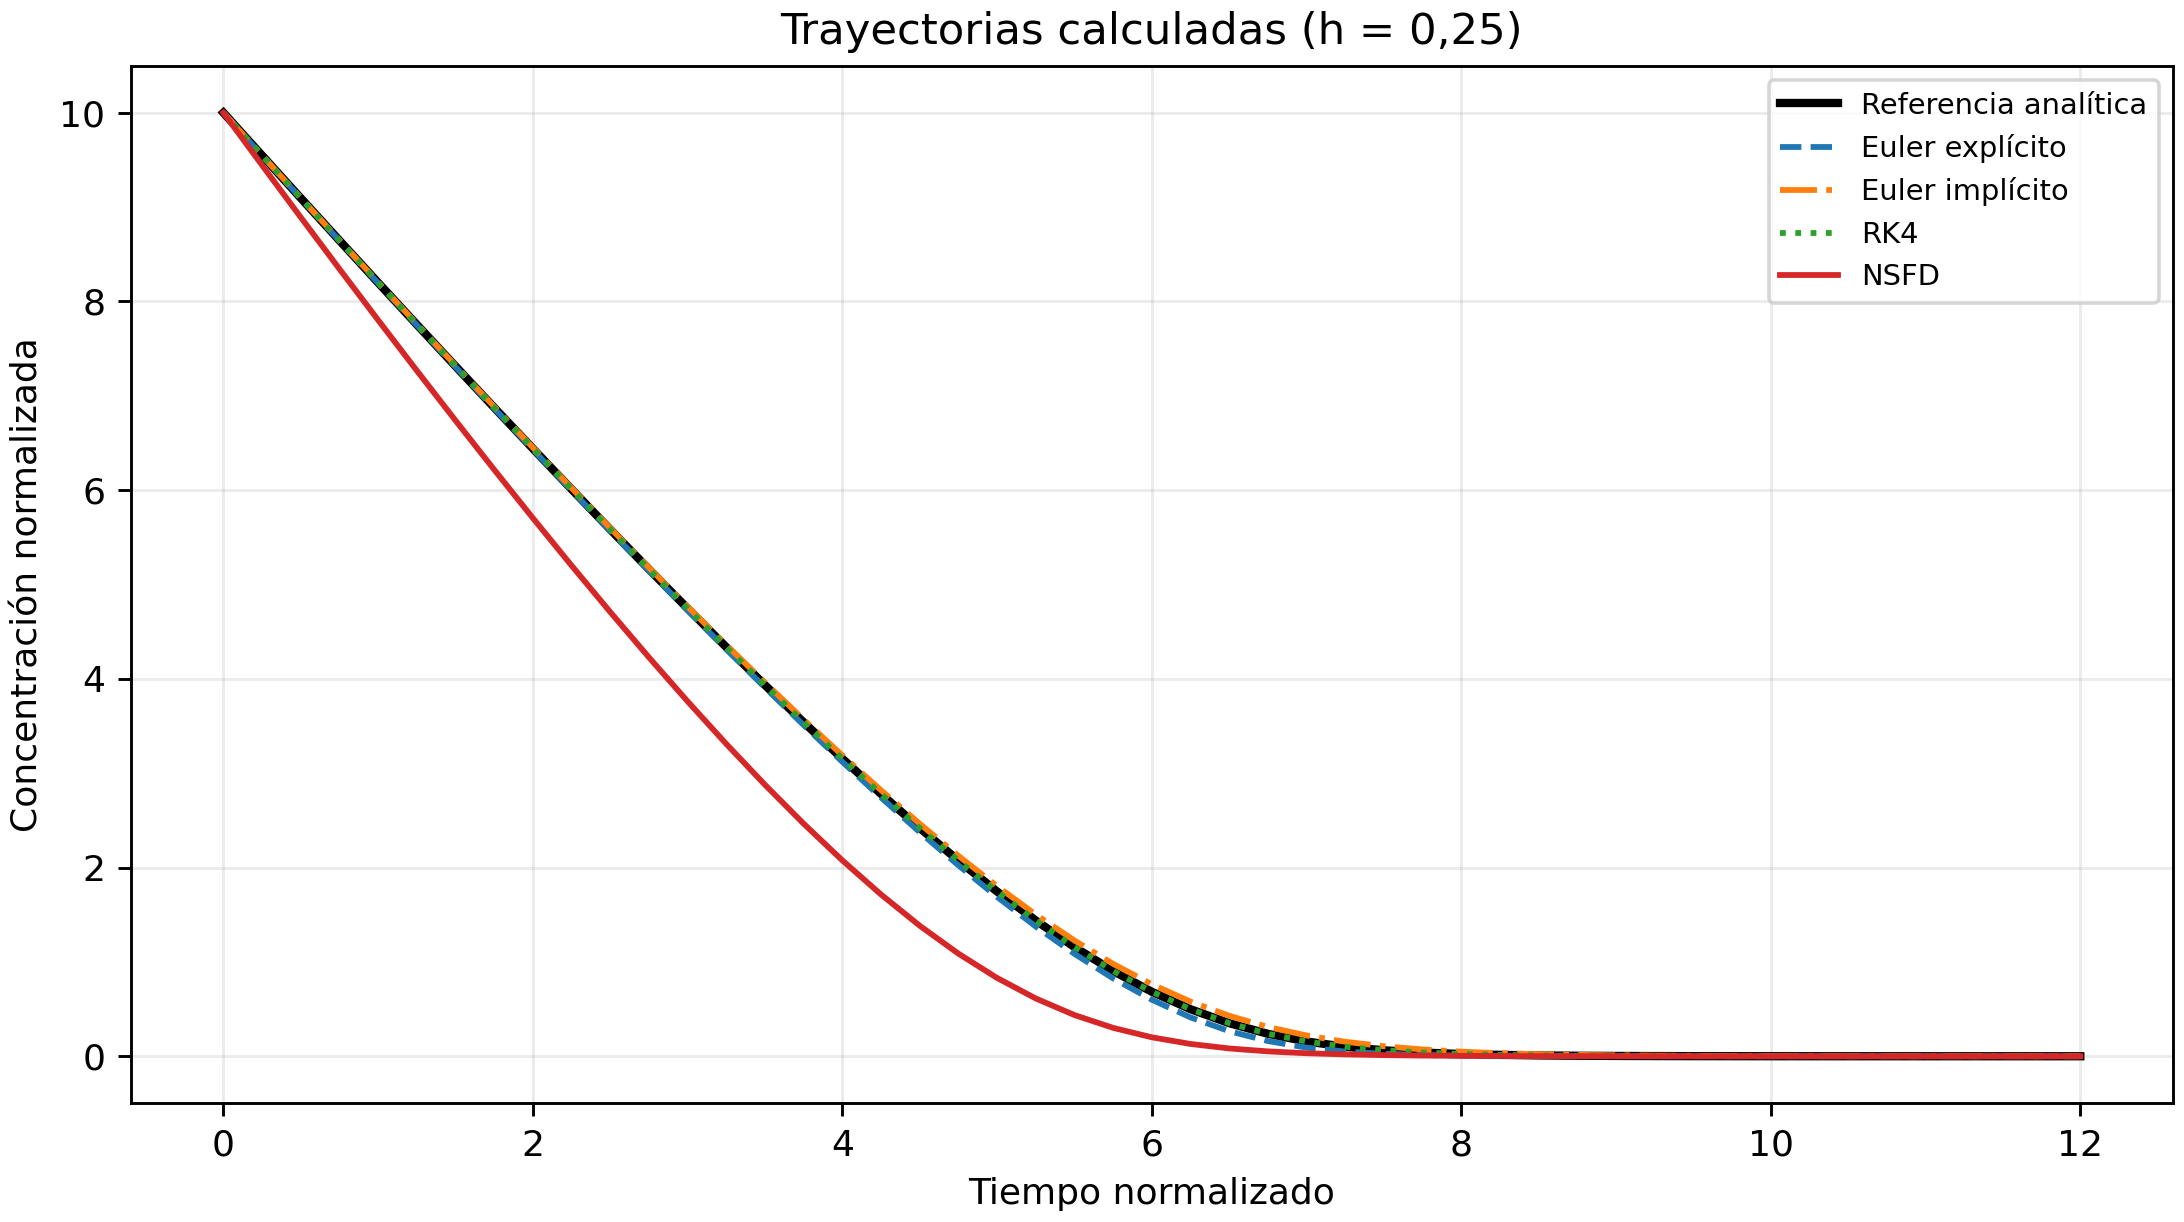
\includegraphics[width=\columnwidth]{figuras/fig1_trayectorias.png}
\caption{Evolución temporal de las concentraciones para $h=0.25$ y comparación con la solución de referencia.}
\label{fig:curvas}
\end{figure}

\begin{figure}[t]
\centering
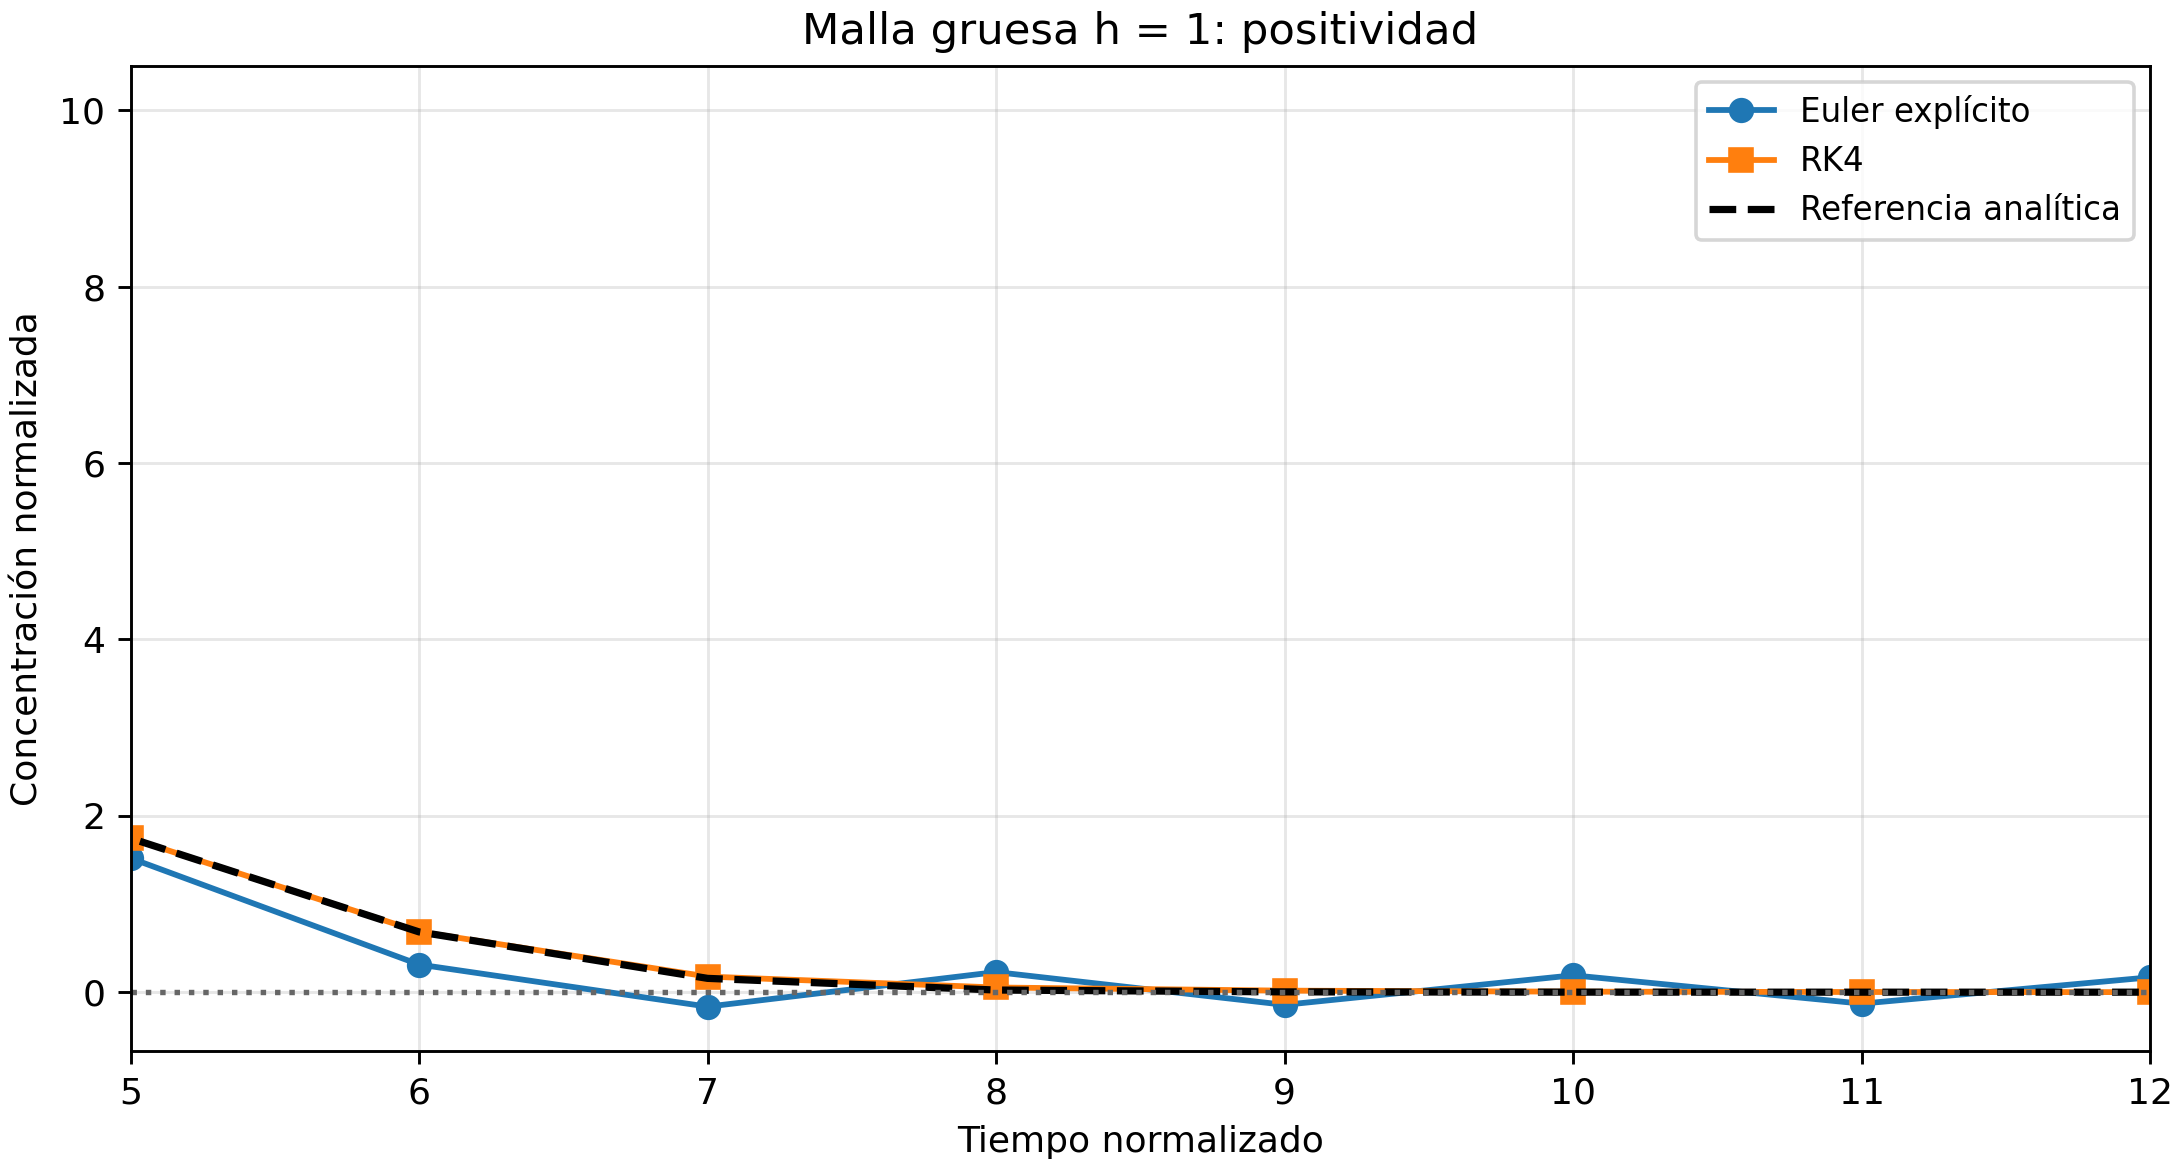
\includegraphics[width=\columnwidth]{figuras/fig3_positividad.png}
\caption{Concentraciones en una malla gruesa ($h=1$). La línea horizontal corresponde al límite $C=0$.}
\label{fig:positividad}
\end{figure}

La Tabla~\ref{tab:auc} resume la exposición acumulada estimada para $h=0.25$, mediante integración compuesta por trapecios. En todas las trayectorias discretas de esta malla, la concentración máxima se obtuvo al inicio: $C_{max}=10$ y $t_{max}=0$. La AUC discrimina mejor la precisión de cada esquema. Los tiempos presentados en la misma tabla son promedios de $300$ ejecuciones completas por método, medidos en un mismo entorno para la malla $h=0.25$. En esta prueba, NSFD registró el menor tiempo medio, seguido de Euler explícito y RK4; Euler implícito necesitó más tiempo debido a la solución no lineal en cada paso.

\begin{table}[t]
\centering
\caption{Exposición numérica y costo para $h=0.25$. La AUC de referencia es $29.999996$. Cada tiempo es el promedio de 300 ejecuciones en el mismo entorno.}
\label{tab:auc}
\begin{tabular}{@{}lrrr@{}}
\toprule
Método & AUC & Error AUC & Tiempo (ms) \\
\midrule
Euler explícito & 29.71344 & 0.28656 & 0.00625 \\
Euler implícito & 30.31239 & 0.31239 & 0.07262 \\
RK4 & 30.00957 & 0.00957 & 0.01045 \\
NSFD & 25.23468 & 4.76531 & 0.00527 \\
\bottomrule
\end{tabular}
\end{table}

Se contrastó además la resolución iterativa de Euler implícito con dos métodos de búsqueda de raíces y la fórmula algebraica positiva equivalente. Para $h=0.25$, la máxima discrepancia entre los resultados fue $8.88\times10^{-16}$. Se acumularon 168 iteraciones en el primer procedimiento y 210 en el segundo, a lo largo de 48 pasos. Estas concordancias respaldan la consistencia algebraica del esquema para la configuración ensayada.

Para analizar la sensibilidad se alteró un solo parámetro respecto al caso base, manteniendo $h=0.25$. La Tabla~\ref{tab:sensibilidad} reúne los errores de los \emph{cuatro métodos} y, en una malla gruesa, el número de concentraciones negativas de los esquemas explícitos. El error de NSFD fue especialmente elevado cuando $K_m$ disminuyó a $0.5$, mientras que RK4 conservó una precisión alta para la malla fina. La positividad no fue uniforme entre escenarios: con $K_m=0.5$ y $h=1$, RK4 produjo seis valores negativos; Euler explícito presentó violaciones en seis de los siete escenarios. Euler implícito y NSFD no presentaron valores negativos en estos casos.

\begin{table*}[t]
\centering
\caption{Sensibilidad unifactorial: error máximo $E_\infty$ para $h=0.25$, y número de valores negativos en la malla $h=1$. Los resultados de los cuatro métodos fueron contrastados con una verificación independiente.}
\label{tab:sensibilidad}
\small
\begin{tabular}{@{}lrrrrrr@{}}
\toprule
Escenario & Euler expl. & Euler impl. & RK4 & NSFD & Neg. E. expl. & Neg. RK4 \\
\midrule
$C_0=5$        & $8.029\!\times\!10^{-2}$ & $7.362\!\times\!10^{-2}$ & $4.713\!\times\!10^{-5}$ & 0.368 & 5 & 0 \\
Base $10,2,1$  & $8.698\!\times\!10^{-2}$ & $8.080\!\times\!10^{-2}$ & $4.706\!\times\!10^{-5}$ & 1.078 & 3 & 0 \\
$C_0=15$       & $8.938\!\times\!10^{-2}$ & $8.317\!\times\!10^{-2}$ & $4.720\!\times\!10^{-5}$ & 1.911 & 2 & 0 \\
$V_{max}=1.5$  & $6.440\!\times\!10^{-2}$ & $6.106\!\times\!10^{-2}$ & $1.389\!\times\!10^{-5}$ & 0.821 & 2 & 0 \\
$V_{max}=2.5$  & $1.099\!\times\!10^{-1}$ & $1.002\!\times\!10^{-1}$ & $1.217\!\times\!10^{-4}$ & 1.326 & 4 & 0 \\
$K_m=0.5$      & $9.435\!\times\!10^{-2}$ & $8.262\!\times\!10^{-2}$ & $4.806\!\times\!10^{-4}$ & 2.631 & 2 & 6 \\
$K_m=2$        & $7.837\!\times\!10^{-2}$ & $7.507\!\times\!10^{-2}$ & $5.101\!\times\!10^{-6}$ & 0.382 & 0 & 0 \\
\bottomrule
\end{tabular}
\end{table*}

\section{Discusión}
\label{discusion}

El contraste con la solución del modelo integrado permite evaluar el error global sin elegir arbitrariamente otro integrador como patrón de comparación. Dentro del intervalo y los pasos examinados, RK4 presentó una convergencia más rápida, acorde con el orden del método descrito por \citet{butcher1996}. Sin embargo, su resultado no debe extrapolarse a todos los parámetros ni a cualquier tamaño de paso, pues el caso $K_m=0.5$ con $h=1$ reveló violaciones de positividad. Esto confirma que el control del error y la conservación de propiedades físicas deben analizarse por separado.

Euler implícito y NSFD conservaron concentraciones no negativas en los escenarios considerados, pero tal comportamiento no implicó la misma precisión. El error de NSFD fue mayor en varias configuraciones, pese a su preservación cualitativa. Esta diferencia concuerda con la necesidad de estudiar las propiedades de cada discretización no estándar particular, en lugar de considerar a todos los esquemas NSFD equivalentes (\citealp{mickens2002,egbelowo2018}). Del mismo modo, el resultado de Euler explícito para pasos gruesos muestra la importancia práctica de imponer criterios de admisibilidad en modelos de eliminación saturable.

Los indicadores de exposición permiten una comparación adicional, pero deben interpretarse teniendo en cuenta que el cálculo por la regla compuesta del trapecio agrega un error de cuadratura que no coincide necesariamente con el orden del integrador temporal. \citet{purves1992} analizó precisamente la influencia del procedimiento de integración en los indicadores farmacocinéticos. La variación de los parámetros, además, modifica el comportamiento de los errores sin que esto convierta los valores normalizados utilizados aquí en predicciones clínicas (\citealp{tang2007,wagner1973}).

Respecto al costo computacional, los esquemas directos realizan menos evaluaciones por paso; RK4 utiliza cuatro evaluaciones de la función de evolución y Euler implícito requiere resolver una ecuación no lineal en cada avance temporal. Con $h=0.25$, las medias registradas fueron $0.00527$ ms para NSFD, $0.00625$ ms para Euler explícito, $0.01045$ ms para RK4 y $0.07262$ ms para Euler implícito. En estas condiciones, NSFD fue el menos costoso en tiempo, aunque tuvo errores superiores a los de los otros métodos. Euler implícito tardó aproximadamente 13.8 veces lo que NSFD. Estas diferencias reflejan el costo observado en esta ejecución y no necesariamente se mantienen en otras máquinas o con otros tamaños de paso.

\setlength{\bibsep}{0pt}
\begin{thebibliography}{99}
\bibitem[Butcher(1996)]{butcher1996}
Butcher, J. C. (1996). A history of Runge--Kutta methods. \emph{Applied Numerical Mathematics, 20}(3), 247--260. \url{https://doi.org/10.1016/0168-9274(95)00108-5}
\bibitem[Egbelowo(2018)]{egbelowo2018}
Egbelowo, O. (2018). Nonlinear elimination of drugs in one-compartment pharmacokinetic models: Nonstandard finite difference approach for various routes of administration. \emph{Mathematical and Computational Applications, 23}(2), 27. \url{https://doi.org/10.3390/mca23020027}
\bibitem[Egbelowo et~al.(2017)Egbelowo, Harley, and Jacobs]{egbelowo2017}
Egbelowo, O., Harley, C., \& Jacobs, B. (2017). Nonstandard finite difference method applied to a linear pharmacokinetics model. \emph{Bioengineering, 4}(2), 40. \url{https://doi.org/10.3390/bioengineering4020040}
\bibitem[Mickens(2002)]{mickens2002}
Mickens, R. (2002). Nonstandard finite difference schemes for differential equations. \emph{Journal of Difference Equations and Applications, 8}(9), 823--847. \url{https://doi.org/10.1080/1023619021000000807}
\bibitem[Purves(1992)]{purves1992}
Purves, R. D. (1992). Optimum numerical integration methods for estimation of area-under-the-curve (AUC) and area-under-the-moment-curve (AUMC). \emph{Journal of Pharmacokinetics and Biopharmaceutics, 20}(3), 211--226. \url{https://doi.org/10.1007/BF01062525}
\bibitem[Tang and Xiao(2007)]{tang2007}
Tang, S., \& Xiao, Y. (2007). One-compartment model with Michaelis--Menten elimination kinetics and therapeutic window: An analytical approach. \emph{Journal of Pharmacokinetics and Pharmacodynamics, 34}, 807--827. \url{https://doi.org/10.1007/s10928-007-9070-4}
\bibitem[Wagner(1973)]{wagner1973}
Wagner, J. G. (1973). Properties of the Michaelis--Menten equation and its integrated form which are useful in pharmacokinetics. \emph{Journal of Pharmacokinetics and Biopharmaceutics, 1}(2), 103--121.\enspace\url{https://doi.org/10.1007/BF01059625}
\bibitem[Yang and Liu(2021)]{yang2021}
Yang, H., \& Liu, Y. (2021). Uncertain pharmacokinetic model based on uncertain differential equation. \emph{Applied Mathematics and Computation, 409}, 126118. \url{https://doi.org/10.1016/j.amc.2021.126118}
\end{thebibliography}

\clearpage
\appendix
\section*{Anexo: reproducibilidad y código}
Los métodos están implementados en los archivos \texttt{codigo/Avance3\_Farmacocinetica.mlx} y \texttt{codigo/Avance3\_Farmacocinetica.m}, ejecutables en MATLAB. Se conservan las plantillas originales de clase, junto con las tablas y figuras del estudio. Los resultados contrastados de sensibilidad y tiempos medios se encuentran, respectivamente, en \texttt{datos/tabla\_sensibilidad\_metodos\_matlab.csv} y \texttt{datos/tabla\_tiempos\_matlab.csv}. Cada tiempo corresponde a una malla con $h=0.25$ y al promedio de $300$ ejecuciones. En el mismo directorio se conserva la tabla de errores del estudio de convergencia.

\noindent\textbf{Repositorio del grupo:}\\
\url{https://github.com/GDS1474-utec/avance3-metodos-numericos-grupo6}



\end{document}
